\section{Unsupervised consensus maximization}

Consensus maximization in a set of features related by a geometric constraint that also contains outliers is an important aspect of an SFM system. The problem consists of finding the largest set of inlier features in a set that is consistent with a geometric constraint. In a 3D vision setting the geometric constraint could be for example a rigid transformation $[\textbf{R}\ \textbf{t}]$, a fundamental matrix $F$ or a homography $H$ that relates pairs of corresponding 3D or 2D points.

A popular algorithm to solve this problem is RANSAC\cite{ransac}, but is however not differentiable and therefore not learnable by a neural network. In this paper\cite{consensus} from 2019 the authors present a differential method to learn consensus maximization in an unsupervised setting. The explanation  of the method in the paper is however very theoretical and non-accessible to master level students. In this section I will try to explain the method with emphasis on ease of understanding and with the mathematical toolbox of an engineering student. I will focus on the method used to extract the parameters of the constraint, as it's not explained by the paper in detail and took a lot of figuring out on my part, especially how to extract the homography.

Consider one of the simplest geometric constraint on a set of corresponding 2D points in subsequent frames of the KITTI dataset, the fundamental matrix $F$. Given a point $u$ in frame 1, and point $v$ in frame 2 they are related in the following way.

 \[
 u^T F v = 0
 \]
 
 To be more explicit the relation can be expressed as follows.
 
\[
\begin{pmatrix}
u_x & u_y & 1 \\
\end{pmatrix}
\begin{pmatrix}
f_{11} & f_{12} & f_{13} \\
f_{21} & f_{22} & f_{23} \\
f_{31} & f_{32} & f_{33} \\
\end{pmatrix}
\begin{pmatrix}
v_x \\
v_y \\
1 \\
\end{pmatrix}
= 0
\]

Multiplication of the two rightmost matrices gives:

\[
\begin{pmatrix}
u_x & u_y & 1 \\
\end{pmatrix}
\begin{pmatrix}
f_{11} v_x + f_{12} v_y + f_{13} \\
f_{21} v_x + f_{22} v_y + f_{23} \\
f_{31} v_x + f_{32} v_y + f_{33} \\
\end{pmatrix}
= 0
\]

Multiplication of the remaining two matrices and grouping the monomials in parentheses for readability gives the following linear equation.

\[
f_{11} (u_x v_x) + f_{12} (u_x v_y) + f_{13} (u_x) +
f_{21} (u_y v_x) + f_{22} (u_y v_y) + f_{23} (u_y) +
f_{31} (v_x) + f_{32} (v_y) + f_{33} (1)
= 0
\]

Now consider a set of $m$ corresponding points that are related by the same fundamental matrix $F$. Place the 9 monomials in the parentheses for all $m$ points in a matrix $ M \in \mathbb{R}^{mx9} $. A matrix of monomials, such as this one, is called a Vandermonde matrix.

\[
M=
\begin{pmatrix}
u_{x,1} v_{x,1} & u_{x,1} v_{y,1} & u_{x,1} & u_{y,1} v_{x,1} & u_{y,1} v_{y,1} & u_{y,1} & v_{x,1} & v_{y,1} & 1 \\
 & & & \vdots & & & & & \\
u_{x,m} v_{x,m} & u_{x,m} v_{y,m} & u_{x,m} & u_{y,m} v_{x,m} & u_{y,m} v_{y,m} & u_{y,m} & v_{x,m} & v_{y,m} & 1 \\
\end{pmatrix}
\]

The constraint is satisfied by all $m$ points if

\[
M
\begin{pmatrix}
f_{11} \\
f_{12} \\
f_{13} \\
f_{21} \\
f_{22} \\
f_{23} \\
f_{31} \\
f_{32} \\
f_{33} \\
\end{pmatrix}
=
\begin{pmatrix}
0 \\
\vdots \\
0 \\
\end{pmatrix}
^{mx1}
\]

Now the solution $\textbf{f}$ should look very familiar. The column vector $\textbf{f}$ is in fact the very definition of a nullspace of $M$. This is the key insight in this method of unsupervised consensus maximization. Finding the nullspace of $M$ is done by performing a singular value decomposition, which is a differentiable operation.

\[
U\Sigma V^T=M
\]

The nullspace will be the last column vector of $V \in \mathbb{R}^{9x9}$ and the last singular value $\sigma_9$ in the diagonal of $\Sigma$ will be zero. This is correct only if the set of corresponding points contains only inliers. If the set contains outliers that can not be related by the gemoetric constraint then the last singular value $\sigma_9$ will be greater than zero. If the inliers and outliers where known they could be represented by a vector $\textbf{w} \in [0,1]^m$ where $ 1 $ means inlier and $ 0 $ means outlier. Now $M$ can be weighted by $\textbf{w}$ which would cancel all rows in $M$ which comes from an outlier pair of points.

\[
\diag(\textbf{w}) M \textbf{f} = \textbf{0}
\] 

The problem of finding the largest set of inliers has now been transformed into finding the weights $\textbf{w}$ such that the last singular value $\sigma_9$ of $\diag(\textbf{w})M$ is near zero, and the sum of the weights should also be large to have as many inliers as possible.

To learn the weight $w \in \textbf{w}$ for each pair of points, the PointNet\cite{pointnet} architecture was used. The pair of points are concatenated into rows of a $ X \in \mathbb{R}^{mxn} $ matrix. For 2D points $n = 2+2=4$ and for 3D points $n=3+3=6$. The input $X$ is fed trough the PointNet segmentation network with a single output class, signifying if the point pair is an inlier or not. The key innovation of the PointNet architecture is that it can directly consume point cloud data, as oppose to first transforming the input to a 3D voxel grid or an image. The network is also invariant to the ordering of the points in the input list. Figure \ref{fig:consensus} illustrates the process of feeding the input through pointnet to get the weights, and then applying the weights to the Vandermonde matrix of which we want to minimize the last singular value.

\begin{figure}[H]
	\centering
	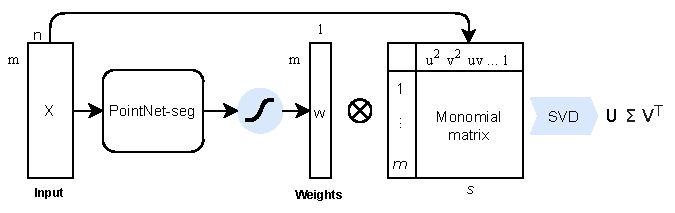
\includegraphics[width=1.0\textwidth]{consensus}
	\caption{}
	\label{fig:consensus}
\end{figure}

Because the fundamental matrix is a constraint expressed by 1 linear equation a basis of only 1  nullspace vector is needed from the singular value decomposition to construct it. But the method can also be used to learn constraints such as a homography or rigid 3D transformation that are constrained by 3 linear equations and therefore require a basis of 3 nullspace vectors. In that case the last 3 singular values from the SVD should be minimized in the loss function.

In the following sections the method used to extract the homography from the basis vectors will be explained. Two points that are related by a homography is expressed as follows. The monomials are grouped by parentheses.

\[
u \times Hv=0 \rightarrow
\]
\[
[u]_{\times} Hv=0 \rightarrow
\]
\[
\begin{pmatrix}
0 & -1 & u_y \\
1 & 0 & -u_x \\
-u_y & u_x & 0 \\
\end{pmatrix}
\begin{pmatrix}
h_{11} & h_{12} & h_{13} \\
h_{21} & h_{22} & h_{23} \\
h_{31} & h_{32} & h_{33} \\
\end{pmatrix}
\begin{pmatrix}
v_x \\
v_y \\
1 \\
\end{pmatrix}
=
\begin{pmatrix}
0 \\
0 \\
0 \\
\end{pmatrix}
\rightarrow
\]
\[
\begin{cases}
-h_{21} (v_x) \ \ \ \ - h_{22} (v_y) \ \ \ \ - h_{23} (1) \ \ \ + h_{31} (v_x u_y) + h_{32} (v_y u_y) + h_{33} (u_y) = 0 \\
\ \ h_{11} (v_x) \ \ \ \ \ + h_{12} (v_y) \ \ \ \ + h_{13} (1) \ \ -h_{31} (v_x u_x) -h_{32} (v_y u_x) - h_{33} (u_x) = 0 \\
-h_{11} (v_x u_y) -h_{12} (v_y u_y) -h_{13} (u_y) + h_{21} (v_x u_x) + h_{22} (v_y u_x) + h_{23} (u_x) = 0 \\
\end{cases}
\]

The monomials are the same as for the fundamental constraint, which means that the same Vandermonde matrix $M$ can be used. But because an homography is constrained by $r=3$ linear equations the last 3 singular values of the SVD should be minimized during training.

Extract 3 basis vectors from the nullspace which will be the 3 rightmost columns of $ V $ in the SVD of $diag(\textbf{w})M$.

\[
B = 
\begin{pmatrix}
\textbf{v}_7 & \textbf{v}_8 & \textbf{v}_9
\end{pmatrix}
\in \mathbb{R}^{9x3}
\]

The 3 linear equations of the homography are tangled which means that the elements of $B$ can not be directly mapped onto the elements in $H$. Notice that the first equation of $H$ does not contain $u_y$ and the second equation of $H$ does not contain $u_x$. We can exploit this fact to perform a change of basis from $B \in \mathbb{R}^{9x3}$ to $B' \in \mathbb{R}^{9x2}$ that should have the following structure.

\begin{center}
\begin{tabular}{ c c c }
	Monomial & Structure of $B'$ & Corresponding element in $H$ \\
	$u_x v_x$ & \multirow{9}{*}{
$\begin{pmatrix}
	0 & . \\
	0 & . \\
	0 & . \\
	. & 0 \\
	. & 0 \\
	. & 0 \\
	. & . \\
	. & . \\
	. & . \\
\end{pmatrix}$
} & \multirow{9}{*}{
$\begin{pmatrix}
 & h_{31} \\
 & h_{32} \\
 & h_{33} \\
h_{31} &   \\
h_{32} &   \\
h_{33} &   \\
h_{21} & h_{11} \\
h_{22} & h_{12} \\
h_{23} & h_{13} \\
\end{pmatrix}$
} \\
	$u_x v_y$ & \\
	$u_x \ \ \ \ $ & \\    
	\hline
	$u_y v_x$ & \\
	$u_y v_y$ & \\
	$u_y \ \ \ \ $ & \\    
	\hline
	$\ \ \ \ v_x$ & \\
	$\ \ \ \ v_y$ & \\
	$\ \ \ \ 1$ & \\
\end{tabular}
\end{center}

To perform the change of basis to get the structure of $B'$ we use the nullspace $\textbf{n}_1 \in \mathbb{R}^{3\times 1}$ of rows 1, 2 and 3 from $B$, and the nullspace $\textbf{n}_2 \in \mathbb{R}^{3x1}$ of row 4, 5, 6 from $B$.

\[
A_1 = 
\begin{pmatrix}
b_{11} & b_{12} & b_{13} \\
b_{21} & b_{22} & b_{23} \\
b_{31} & b_{32} & b_{33} \\
\end{pmatrix},
A_2 = 
\begin{pmatrix}
b_{41} & b_{42} & b_{43} \\
b_{51} & b_{52} & b_{53} \\
b_{61} & b_{62} & b_{63} \\
\end{pmatrix}
\]
\[
\textbf{n}_1 = \textit{"rightmost column of right-singular vectors of A1"}
\]
\[
\textbf{n}_2 = \textit{"rightmost column of right-singular vectors of A2"}
\]
\[
\textbf{b}^{n_1} = B\textbf{n}_1
\]
\[
\textbf{b}^{n_2} = B\textbf{n}_2
\]

Now the $\textbf{b}^{n_1}$ and $\textbf{b}^{n_2}$ basis vectors will have the following structure as desired.

\[
\textbf{b}^{n_1} =
\begin{pmatrix}
0 \\
0 \\
0 \\
. \\
. \\
. \\
. \\
. \\
. \\
\end{pmatrix},
\textbf{b}^{n_2} =
\begin{pmatrix}
. \\
. \\
. \\
0 \\
0 \\
0 \\
. \\
. \\
. \\
\end{pmatrix},
\]

The basis vectors have zeros at the correct place. The next step is to adjust the scale so that row 4, 5 and 6 of $\textbf{b}^{n_1}$ and row 1, 2 and 3 of $\textbf{b}^{n_2}$ have the same norm because they both represent the same elements $h_{31}$, $h_{32}$ and $h_{33}$. We also make sure they have the same sign.

\[
s = \sign(b^{n_2}_1 + b^{n_2}_2 + b^{n_2}_3) \sign(b^{n_1}_4 + b^{n_1}_5 + b^{n_1}_6)
\]

$s$ will be -1 if they have different signs, or 1 if they are the same sign.

\[
B'=
\begin{pmatrix}
\textbf{b}^{n_1} / \norm{(b^{n_1}_4 \ b^{n_1}_5 \ b^{n_1}_6)
} &
\textbf{b}^{n_2} / \norm{(b^{n_2}_1 \ b^{n_2}_2 \ b^{n_2}_3)} s
\end{pmatrix}
\in \mathbb{R}^{9x2}
\]

It is now possible to assign the elements of $H$ by pattern matching.

\[
H=
\begin{pmatrix}
\ \ b'_{72} & \ \ b'_{82} & \ \ b'_{92} \\
\ \ b'_{71} & \ \ b'_{81} & \ \ b'_{91} \\
-b'_{41} & -b'_{51} & -b'_{61} \\
\end{pmatrix}
\]

The method not only works for predicting the fundamental or homographic relationship between points, but can also be used for 3D rigid transformations.

\[
v=Ru+t \rightarrow
\]
\[
Ru+t-v=0 \rightarrow
\]
\[
\begin{pmatrix}
r_{11} & r_{12} & r_{13} \\
r_{21} & r_{22} & r_{23} \\
r_{31} & r_{32} & r_{33} \\
\end{pmatrix}
\begin{pmatrix}
u_x \\
u_y \\
y_z \\
\end{pmatrix}
+
\begin{pmatrix}
t_x \\
t_y \\
t_z \\
\end{pmatrix}
-
\begin{pmatrix}
v_x \\
v_y \\
v_z \\
\end{pmatrix}
=
\begin{pmatrix}
0 \\
0 \\
0 \\
\end{pmatrix}
\rightarrow
\]
\[
\begin{cases}
r_{11} (u_x) + r_{12} (u_y) + r_{13} (u_z) + t_x (1) - (v_y) = 0 \\
r_{21} (u_x) + r_{22} (u_y) + r_{23} (u_z) + t_y (1) - (v_x) = 0 \\
r_{31} (u_x) + r_{32} (u_y) + r_{33} (u_z) + t_z (1) - (v_z) = 0 \\
\end{cases}
\]

The monomials in the parentheses form the following Vandermonde matrix.

\[
M=
\begin{pmatrix}
u_{x,1} & u_{y,1} & u_{z,1} & v_{x,1} & v_{y,1} & v_{z,1} & 1 \\
 & & & \vdots & & & \\
u_{x,m} & u_{y,m} & u_{z,m} & v_{x,m} & v_{y,m} & v_{z,m} & 1 \\
\end{pmatrix}
\]

The constraint of $r=3$ linear equations is satisfied for all inliers if

\[
\diag(\textbf{w})
M
\begin{pmatrix}
r_{11} & r_{21} & r_{31} \\
r_{12} & r_{22} & r_{32} \\
r_{13} & r_{23} & r_{33} \\
-1 & 0 & 0 \\
0 & -1 & 0 \\
0 & 0 & -1 \\
t_x & t_y & t_z \\
\end{pmatrix}
=
\begin{pmatrix}
0 \\
\vdots \\
0 \\
\end{pmatrix}
^{mx1}
\]

Similar to before $R$ and $t$ is extracted from the null vectors of $\diag(\textbf{w})M$. The null vectors are the 3 rightmost singular vectors in the SVD. The 3 null vectors form a basis matrix $B$ on which a change of basis is performed to untangle the components $v_x$, $v_y$ and $v_z$ into a new structure $B'$ where $R$ and $t$ are easy to extract.

\begin{center}
	\begin{tabular}{ c c c }
		Monomial & Structure of $B'$ &  \\
		$u_x$ & \multirow{7}{*}{
			$\begin{pmatrix}
			r_{11} & r_{21} & r_{31} \\
			r_{12} & r_{22} & r_{32} \\
			r_{13} & r_{23} & r_{33} \\
			-1 & 0 & 0 \\
			0 & -1 & 0 \\
			0 & 0 & -1 \\
			t_x & t_y & t_z \\
			\end{pmatrix}$
		} \\
		$u_y$ & \\
		$u_z$ & \\    
		\hline
		$v_x$ & \\
		$v_y$ & \\
		$v_z$ & \\    
		\hline
		$1$ & \\
	\end{tabular}
\end{center}

\[
B'=
-
\begin{pmatrix}
b_{41} & b_{42} & b_{43} \\
b_{51} & b_{52} & b_{53} \\
b_{61} & b_{62} & b_{63} \\
\end{pmatrix}^{-1}
\begin{pmatrix}
b_{11} & b_{12} & b_{13} \\
b_{21} & b_{22} & b_{23} \\
b_{31} & b_{32} & b_{33} \\
b_{41} & b_{42} & b_{43} \\
b_{51} & b_{52} & b_{53} \\
b_{61} & b_{62} & b_{63} \\
b_{71} & b_{72} & b_{73} \\
\end{pmatrix}
=
\begin{pmatrix}
r_{11} & r_{21} & r_{31} \\
r_{12} & r_{22} & r_{32} \\
r_{13} & r_{23} & r_{33} \\
-1 & 0 & 0 \\
0 & -1 & 0 \\
0 & 0 & -1 \\
t_x & t_y & t_z \\
\end{pmatrix}
\]

However this holds for any affine transformation, to enforce the rotation manifold constraint an additional regularizer loss term is added.

\[
\mathcal{L}_r=\log(1 + || RR^T - I_{3\times3} ||)
\]

\subsection{Improving training convergence}

After some initial attempts at training the consensus maximization network for hagiographies on the output of the keypoint network, it was clear that it was next to impossible to get the training to converge on a good solution. Applying some additional techniques not described in the original paper resolved the issue.

Firstly the points should be transformed into a different basis before they are fed into the consensus maximization network. The change of basis ensures that the coordinates are scaled so that their maximum magnitude is 1, and the origin is centered in the middle of the image and not in the top left corner.

\[
G=
\begin{pmatrix}
W & 0 & W/2 \\
0 & W & H/2 \\
0 & 0 & 1 \\
\end{pmatrix}
\]
\[
p' = G^{-1} p
\]
Where $p$ is the output point from the keypoint network, $W$ and $H$ is the width and height of the image respectively, and $p'$ is the new altered point used as input. The homography $H$ predicted by the consensus maximization network will be in this new basis $G$ and needs to be altered in order to use it in our standard pixel coordinate basis as follows.

\[
H' = G H G^{-1}
\]

The second method to improve convergence during training is to normalize the rows of the Vandermonde matrix as follows.

\[
M_n' = \frac{M_n}{||M_n||}
\]

For all $n$ rows of the Vandermonde matrix $M$.





